\section{Dijkstra - Algorithmus}

\begin{frame}
	\begin{block}{Erweiterung der Knoten um ...}
		\begin{itemize}
			\item<2-> einen Schätzwert.
			\item<3-> einen Vorgänger.
		\end{itemize}
	\end{block}

	\begin{block}<4->{Einschränkung der Kanten}
		\visible<5>{Eine Kante darf nur ein positives Gewicht besitzen.}
	\end{block}
\end{frame}

\begin{frame}
	\begin{block}<1->{white node}
		Ein ``white node'' ist ein Knoten über den weder ein Schätzwert noch ein Vorgänger bekannt ist.
	\end{block}
	\begin{block}<2->{grey node}
		Ein ``grey node'' ist ein Knoten zu dem bereits ein Weg gefunden wurde. Er besitzt also einen Schätzwert und Nachfolger. Diese müssen aber noch nicht optimal sein.
	\end{block}
	\begin{block}<3->{black node}
		Ein ``black node'' ist ein Knoten zu dem bereits der optimale Weg gefunden wurde.
	\end{block}
\end{frame}

\begin{frame}
	\begin{block}{Berechnung von Knotenwerten}
		Der Schätzwert $S_A$ eines Knotens $K_A$ kann berechnet werden, wenn es einen Knoten $K_V$ gibt, dessen Schätzwert $S_V$ bekannt ist und eine gerichtete Kante von $K_V$ nach $K_A$ mit bekannten Gewichtung $g$ existiert.
	\end{block}
	\vfill
	Berechnung: $S_A = S_V + g$
\end{frame}

\begin{frame}
	\begin{block}{Initialisierung}
		\begin{itemize}
			\item<2-> Der Startknoten ist ein ``black node'' mit dem Schätzwert 0. Einen Vorgänger besitzt der Startknoten nicht.
			\item<3-> Alle seine Nachfolgerknoten werden berechnet. Sie sind somit alle ``grey nodes''.
		\end{itemize}
	\end{block}
\end{frame}

\begin{frame}
	\begin{block}{Schritt}
		\begin{itemize}
			\item<2-> Der ``grey node'' mit dem niedrigsten Schätzwert wird gesucht.
			\item<3-> Dieser ``grey node'' wird ab sofort als ``black node'' angesehen.
			\item<4-> Alle Nachfolgerknoten dieses Knotens werden berechnet. Falls die Nachfolger bereits einen Schätzwert hat wird der niedrigere Wert dem Knoten zugeordnet (relaxieren), der Vorgänger wird dabei auch geändert.
		\end{itemize}
	\end{block}
\end{frame}

\begin{frame}
	\begin{block}{Ende}
		\begin{itemize}
			\item<2-> Wenn der Zielknoten ein ``black node'' ist, so hat man den idealen Weg vom Startknoten zum Endknoten gefunden.
		\end{itemize}
	\end{block}
\end{frame}

\begin{frame}
	\only<1>{
		\begin{figure}
			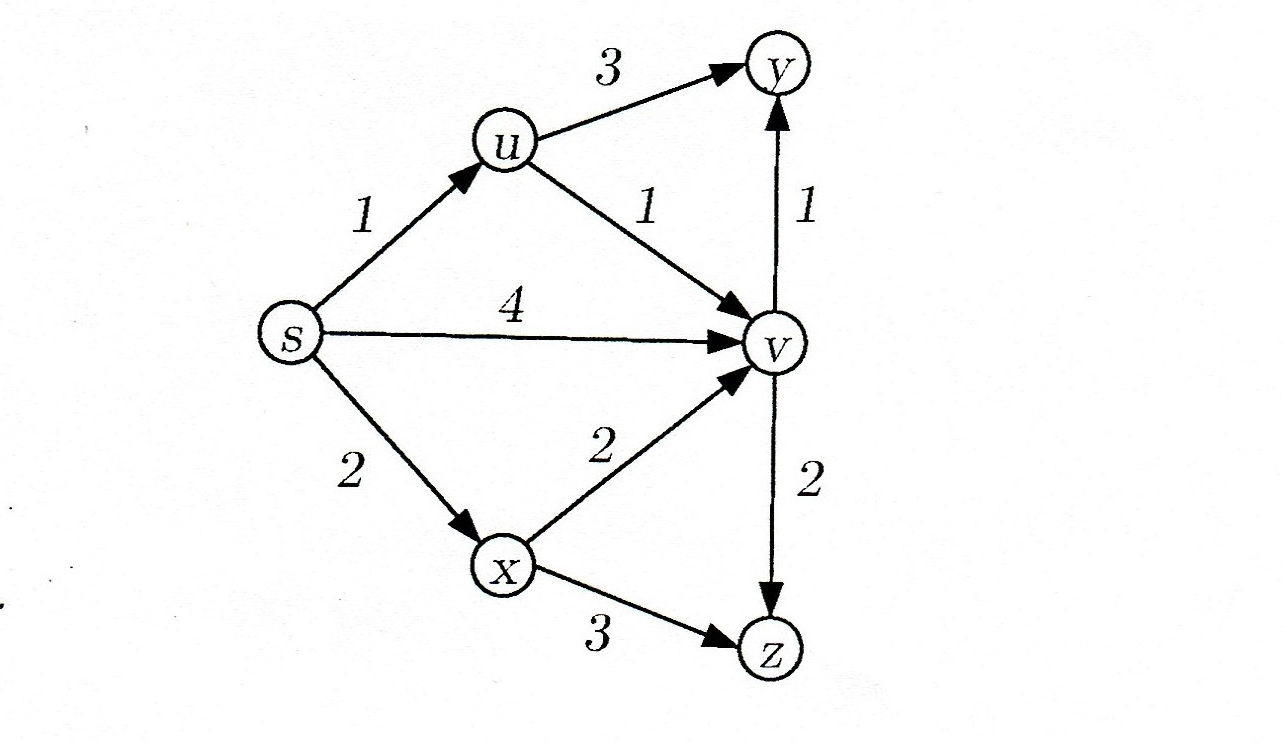
\includegraphics[scale=0.23]{./pictures/00_Graph}
			\caption{Pr. Dr. Schmitz Algorithmendesign}
		\end{figure}
	}
	\only<2>{
		\begin{figure}
			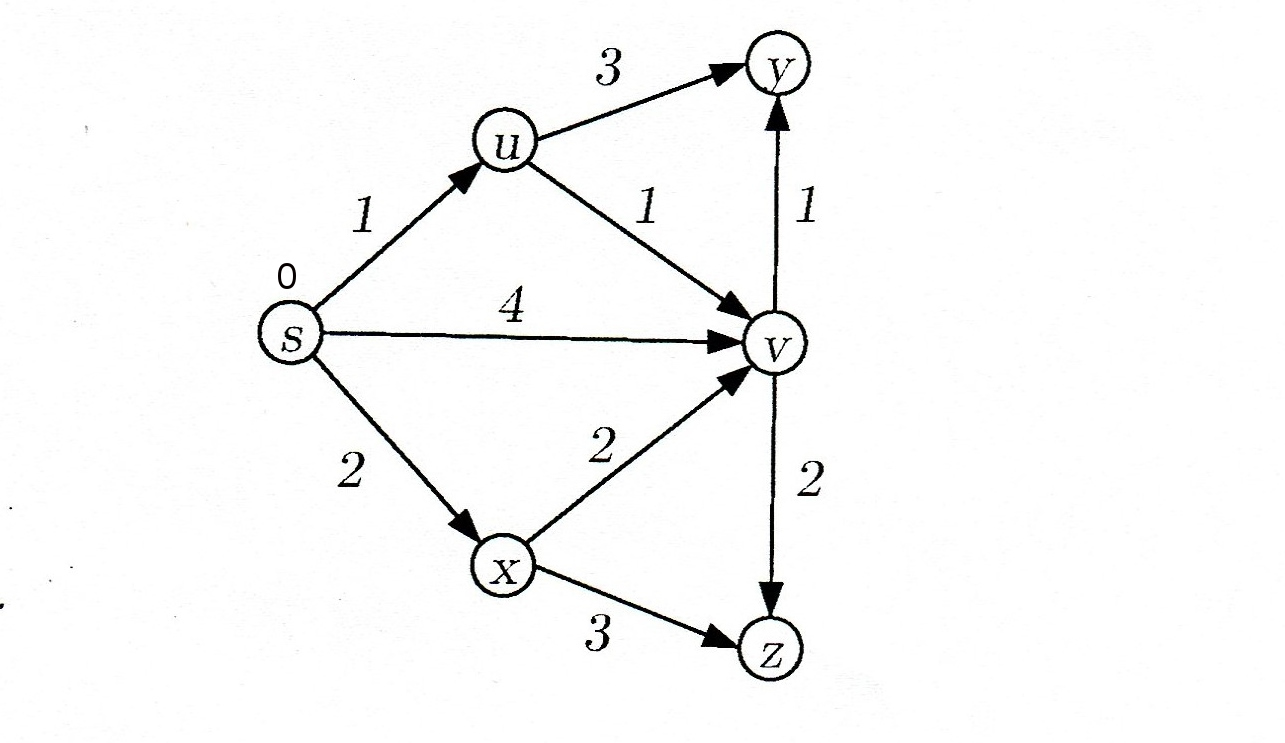
\includegraphics[scale=0.23]{./pictures/01_Graph}
			\caption{Pr. Dr. Schmitz Algorithmendesign}
		\end{figure}
	}
	\only<3>{
		\begin{figure}
			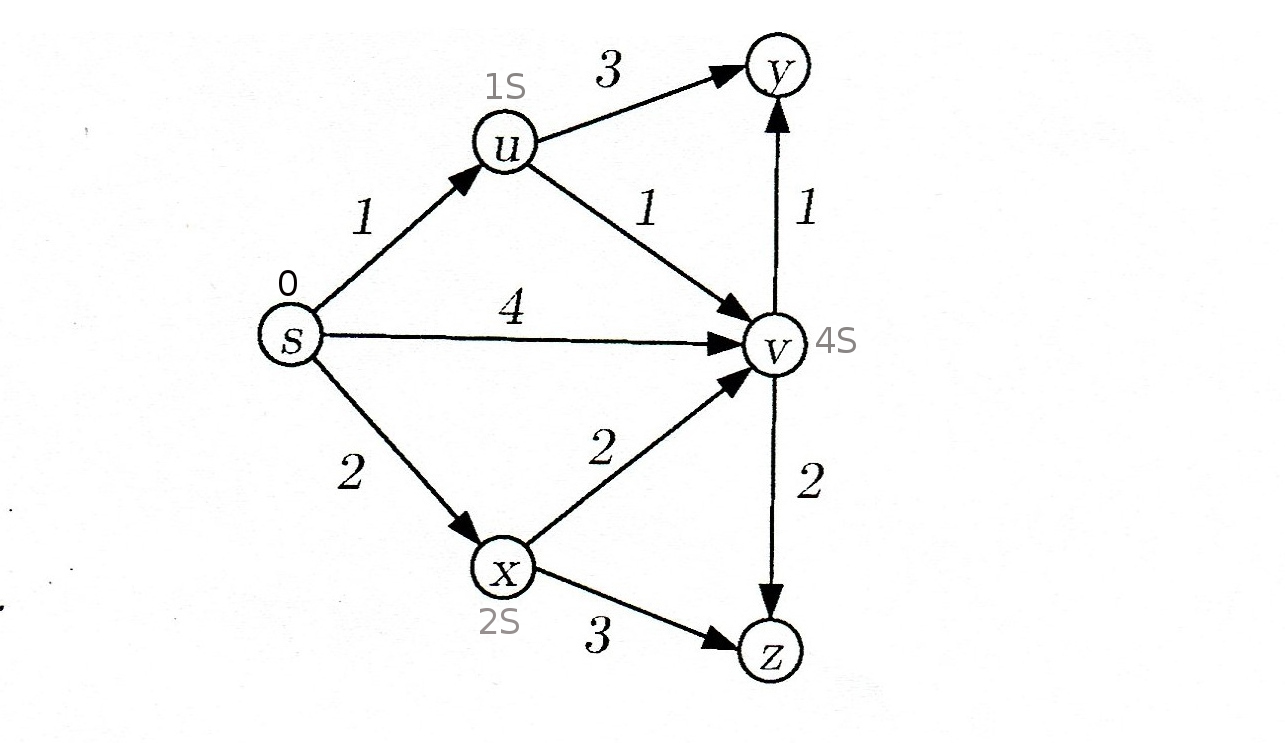
\includegraphics[scale=0.23]{./pictures/02_Graph}
			\caption{Pr. Dr. Schmitz Algorithmendesign}
		\end{figure}
	}
	\only<4>{
		\begin{figure}
			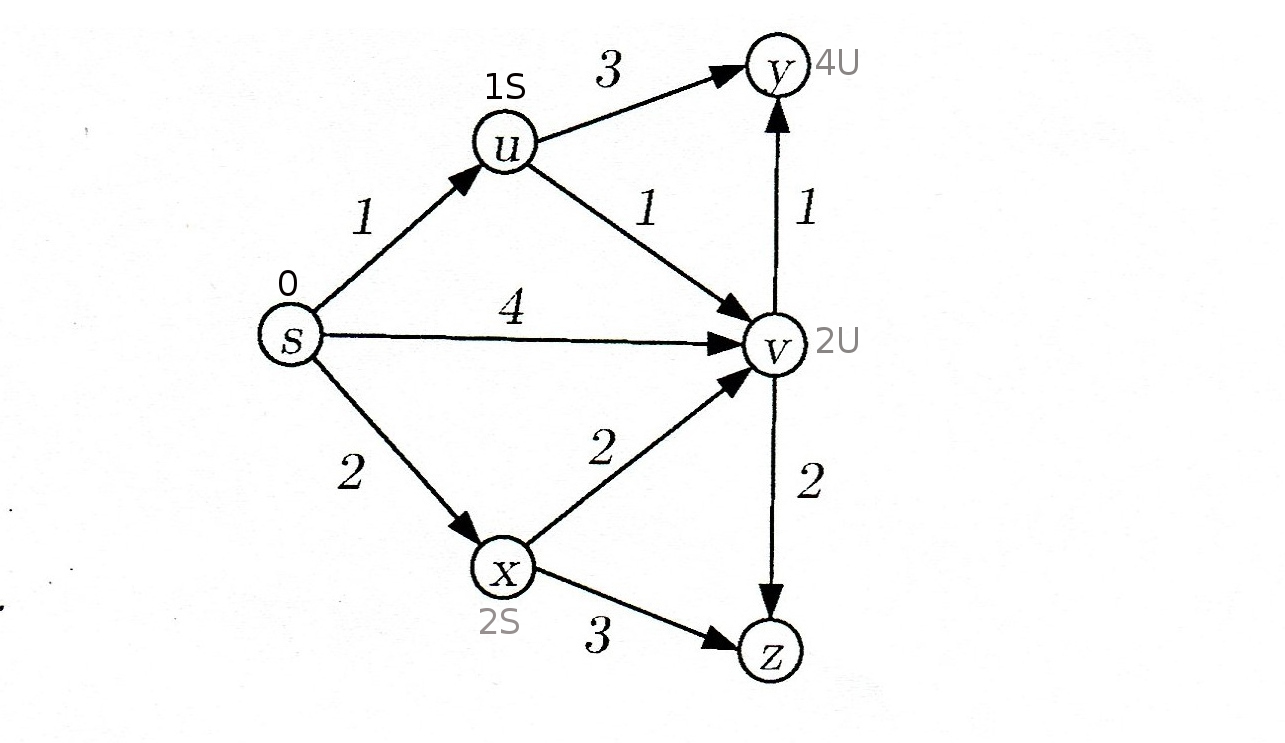
\includegraphics[scale=0.23]{./pictures/03_Graph}
			\caption{Pr. Dr. Schmitz Algorithmendesign}
		\end{figure}
	}
	\only<5>{
		\begin{figure}
			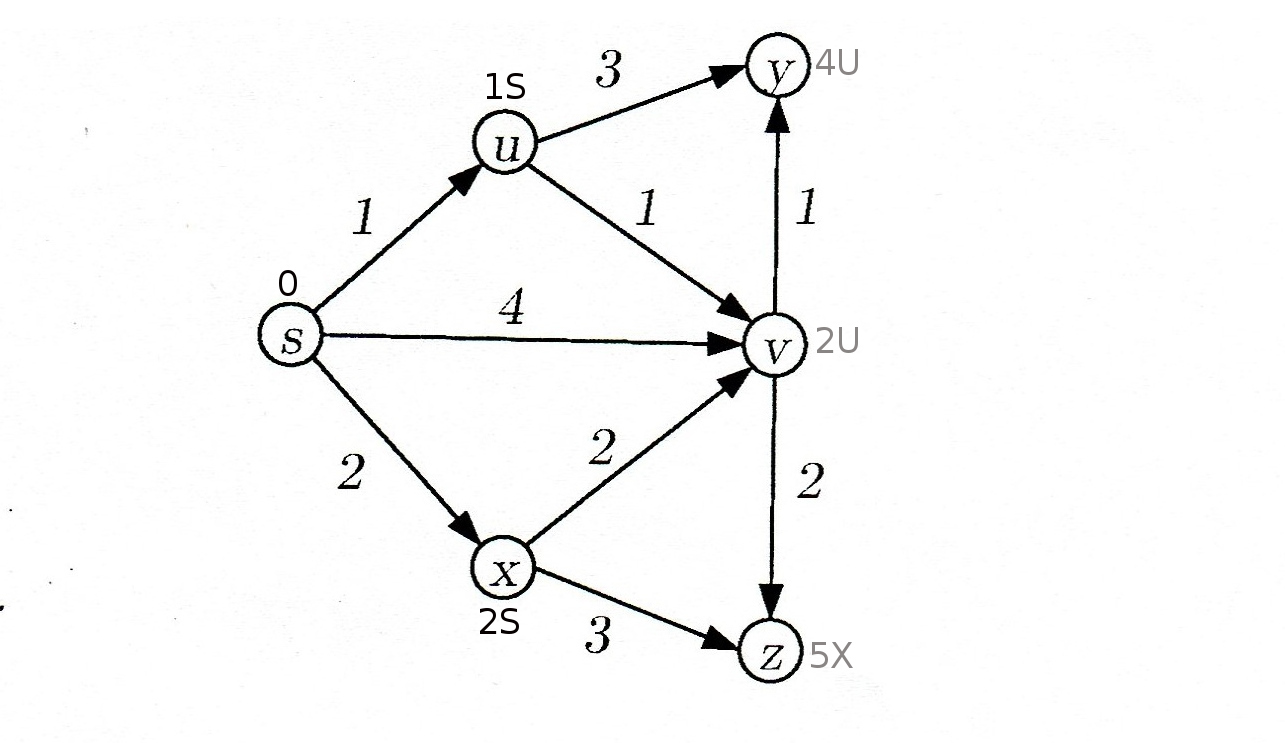
\includegraphics[scale=0.23]{./pictures/04_Graph}
			\caption{Pr. Dr. Schmitz Algorithmendesign}
		\end{figure}
	}
\end{frame}